% =====================================================================
%  단면 그림용 x-y 교차 축 (TikZ)
%  - 별도 라이브러리 없이 동작 (TikZ 기본 기능만 사용)
%  - TikZ 에디터에는 \begin{tikzpicture} ... \end{tikzpicture} 부분만
%    복사해서 붙여넣어도 됩니다.
% =====================================================================
\documentclass[tikz,border=5pt]{standalone}
\definecolor{axiscolor}{HTML}{1F6E8C}   % 축 색 (청록색)
\definecolor{labelcolor}{HTML}{555555}  % 라벨 색 (회색)
\begin{document}

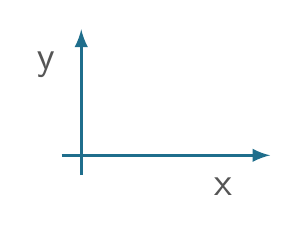
\begin{tikzpicture}[>=latex, line width=1.2pt]
  % 축 길이 / 교차점 밖으로 튀어나온 길이
  \def\xlen{2.4}  \def\ylen{1.6}  \def\tail{0.25}

  % 축
  \draw[->, axiscolor] (-\tail,0) -- (\xlen,0);   % x축
  \draw[->, axiscolor] (0,-\tail) -- (0,\ylen);   % y축

  % 라벨
  \node[labelcolor, font=\sffamily\Large] at (\xlen-0.6,-0.4) {x};
  \node[labelcolor, font=\sffamily\Large] at (-0.45,\ylen-0.45) {y};
\end{tikzpicture}

\end{document}
